\section{Differential Riccati Equation equilibrium}

Since $K(t)=\left(FP(t)H^T+V_{12}\right)\left(FP(t)H^T+V_2\right)^{-1}$, then a constant gain $\bar{K}$ is attainable only if the Differential Riccati Equation possesses an equilibrium point $\bar{P}$.
In addressing the equilibrium of the Differential Riccati Equation, let's delve into the Algebraic Riccati Equation given by:
\[\bar{P}=\left(F\bar{P}F^T+V_1\right)-\left(F\bar{P}H^T+V_{12}\right)\left(H\bar{P}H^T+V_{2}\right)^{-1}\left(F\bar{P}H^T+V_{12}\right)^T\]
This nonlinear matrix static equation, known as Algebraic Riccati Equation, is crucial for determining the existence of a steady-state solution for the Differential Riccati Equation.

To address the equilibrium of the Algebraic Riccati Equation and subsequently the Differential Riccati Equation, we need to prove three critical aspects:
\begin{enumerate}
    \item \textit{Existence}: demonstrating that the Algebraic Riccati Equation possesses semi-definite positive solutions.
    \item \textit{Convergence}: proving the convergence of the Discrete Differential Riccati Equation to $\bar{P}$.
    \item \textit{Stability}: verifying the asymptotic stability of the corresponding Kalman Filter, which is equivalent to ensuring all eigenvalues of $F-\bar{K}H$ lie strictly inside the unit circle.
\end{enumerate}
Although these proofs are challenging, we can rely on two key theorems that provide sufficient conditions for the requested proofs:
\begin{theorem}[First asymptotic Kalman Filter]
    If $V_{12}=0$ and the system is asymptotically stable, then:
\end{theorem}  
\begin{itemize}
    \item \textit{Algebraic Riccati Equation possesses one and only one semi-positive solution $\bar{P}\geq 0$}.
    \item \textit{The corresponding $\bar{K}$ ensures the asymptotic stability of the Kalman Filter}. 
    \item \textit{Differential Riccati Equation converges to $\bar{P}$ for all $P_0\geq 0$}.
\end{itemize}

In the equation for the state:
\[x(t+1)=Fx(t)+Gu(t)+v_1(t) \qquad v_1(t)\sim WN(0,V_1)\]
to introduce another noise source, we require a special type of controllability from the noise $v_1(t)$ since it serves as an input for the states $x(t)$. 
We can reformulate the same equation as:
\[x(t+1)=Fx(t)+Gu(t)+\Gamma_\omega(t) \qquad \omega\sim WN(0,I)\]
Here, $\Gamma_\omega(t)$ represents the factorization of $V_1$, such that $\Gamma\Gamma^T=V_1$.
\begin{example}
    Consider the state equation:
    \[x(t+1)=\dfrac{1}{2}+v_1(t)\qquad v_1(t)\sim WN(0,4)\]
    We can factorize the noise, leading to:
    \[x(t+1)=\dfrac{1}{2}+2\omega(t)\qquad \omega(t)\sim WN(0,1)\]
\end{example}

We can assert that the state is controllable from noise $v_1(t)$ if and only if the controllability matrix is full rank:
\[\text{rank}(R)=\text{rank}\left(\begin{bmatrix} \Gamma & F\Gamma & F^2\Gamma & \cdots & F^n\Gamma \end{bmatrix} \right)=n\]
Here, $n$ denotes the dimension of the state space.
\begin{theorem}[Second asymptotic Kalman Filter]
    If $V_{12}=0$, the pair $(F,H)$ is fully observable, and the pair $(F,\Gamma)$ is fully controllable, then:
\end{theorem}  
\begin{itemize}
    \item \textit{Algebraic Riccati Equation possesses one and only one solution $\bar{P}\geq 0$}. 
    \item \textit{The corresponding $\bar{K}$ ensures the asymptotic stability of the Kalman Filter}. 
    \item \textit{Differential Riccati Equation converges to $\bar{P}$ for all $P_0\geq 0$}. 
\end{itemize}
These theorems are particularly valuable in practice as they allow us to bypass the intricate convergence analysis of the Differential Riccati Equation for systems with $n>1$.
\begin{example}
    Let's consider the system described by:
    \[\mathcal{S}:\begin{cases}
        x(t+1)=\frac{1}{2}x(t)+v_1(t) \\
        t(t)=2x(t)+v_2(t)
    \end{cases}\]
    Here, $v_1\sim WN(0,\frac{19}{20})$ and $v_2\sim WN(0,1)$ are independent noises with $V_{12}=0$. 
    We're tasked with deriving the asymptotic Kalman Filter for one-step prediction and filtering.

    This is a first-order system, with matrices defined as:
    \[F=\begin{bmatrix} \dfrac{1}{2} \end{bmatrix} \quad G=\begin{bmatrix} 0 \end{bmatrix} \quad H=\begin{bmatrix} 2 \end{bmatrix} \quad D=\begin{bmatrix} 0 \end{bmatrix} \]
    The covariance matrices are:
    \[V_1=\frac{19}{20} \quad V_2=1 \quad V_{12}=0\]

    Now, we can proceed to apply the Kalman Filter algorithm: 
    \begin{enumerate}
        \item Let's compute the Differential Riccati Equation using the given formula:
            \[P(t+1)=\left(FP(T)F^T+V_1\right)-\left(FP(t)H^T+V_{12}\right)\left(HP(t)H^T+V_{2}\right)^{-1}\left(FP(t)H^T+V_{12}\right)^T\]
            In our case, we substitute the values:
            \begin{align*}
                P(t+1)  &=\dfrac{1}{4}P(t)+\dfrac{19}{20}-\dfrac{\left(\frac{1}{2}P(t)\cdot 2+0\right)^2}{4P(t)+1} \\
                        &=\dfrac{P(t)^2+\frac{1}{4}P(t)+\frac{19}{5}P(t)+\frac{19}{20}-P(t)^2}{4P(t)+1} \\
                        &=\dfrac{81P(t)+19}{80P(t)+20}
            \end{align*}
        \item Let's compute and solve the Algebraic Riccati Equation:
            \[\bar{P}=\dfrac{81\bar{P}+19}{80\bar{P}+20}\]
            By solving this equation, we find that $\bar{P}$ can take values of $1$ or $-\frac{19}{20}$.
        \item Let's check the convergence using direct analysis of the Differential Riccati Equation and by applying the asymptotic Kalman Filter theorems:
            \begin{itemize}
                \item \textit{Direct analysis}: since we have a first-order system, direct analysis can be performed.
                    We plot the graph of the Differential Riccati Equation in the $P(t)$ and $P(t+1)$ plane: 
                    \begin{itemize}
                        \item The vertical asymptotic value is found by setting $80P(t)+20=0$, obtaining $P(t)=-\frac{1}{4}$. 
                        \item The horizontal asymptotic value is found by letting $P(t)$tend towards infinity, giving $P(t+1)\frac{81}{80}$. 
                        \item The crossing point is found by setting $P(t)=0$, giving $P(t+1)=\frac{19}{20}$. 
                    \end{itemize}
                    \begin{figure}[H]
                        \centering
                        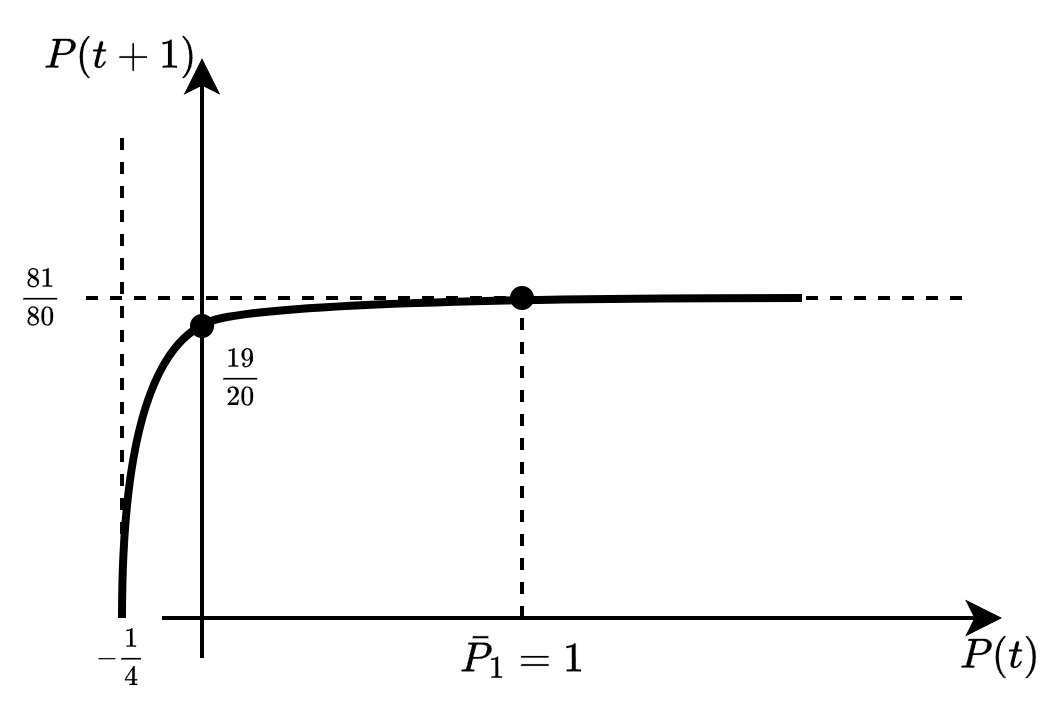
\includegraphics[width=0.4\linewidth]{images/plot.png}
                    \end{figure}
                    Upon zooming in on $\bar{P}_1$ and adding some points before and after, we observe convergence to  $\bar{P}_1$. 
                    \begin{figure}[H]
                        \centering
                        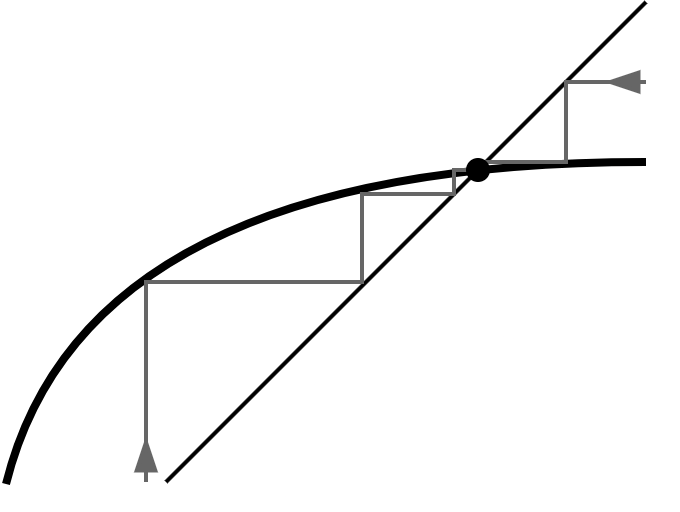
\includegraphics[width=0.3\linewidth]{images/plot1.png}
                    \end{figure}
                \item Given that $V_{12}=0$ and the eigenvalue is $\frac{1}{2}$ (indicating asymptotic stability), the first theorem holds true.
                    Additionally, the observability matrix $O=\begin{bmatrix} 0 \end{bmatrix}$ has rank one, indicating full observability. 
                    Similarly, the reachability matrix $O=\begin{bmatrix} \Gamma \end{bmatrix}=\begin{bmatrix} \sqrt{\frac{19}{20}} \end{bmatrix}$ has rank one, implying full controllability from noise.
                    Consequently, the second theorem is also valid. 
                    Therefore, we can conclude that:
                    \begin{itemize}
                        \item The Algebraic Riccati Equation has one and only one solution.
                        \item The Differential Riccati Equation converges to $\bar{P}$ for each initial $P_0$. 
                        \item The corresponding Kalman Filter is asymptotically stable.
                    \end{itemize}
            \end{itemize}
        \item Let's compute the steady-state Kalman gain $\bar{K}$ using the formula:
            \[\bar{K}=\left(F\bar{P}H^T+V_{12}\right)\left(H\bar{P}H^T+V_2\right)^{-1}=\dfrac{1}{5}\]
            Now, let's check the asymptotic stability of the Kalman Filter:
            \[F-\bar{K}H=\dfrac{1}{2}-\dfrac{1}{5}\cdot 2=\dfrac{1}{20}\]
            Since the resulting value is $\frac{1}{20}$, which is less than 1 in absolute value, the Kalman Filter is asymptotically stable. 
        \item The block scheme of the Kalman Filter is illustrated as follows:
            \begin{figure}[H]
                \centering
                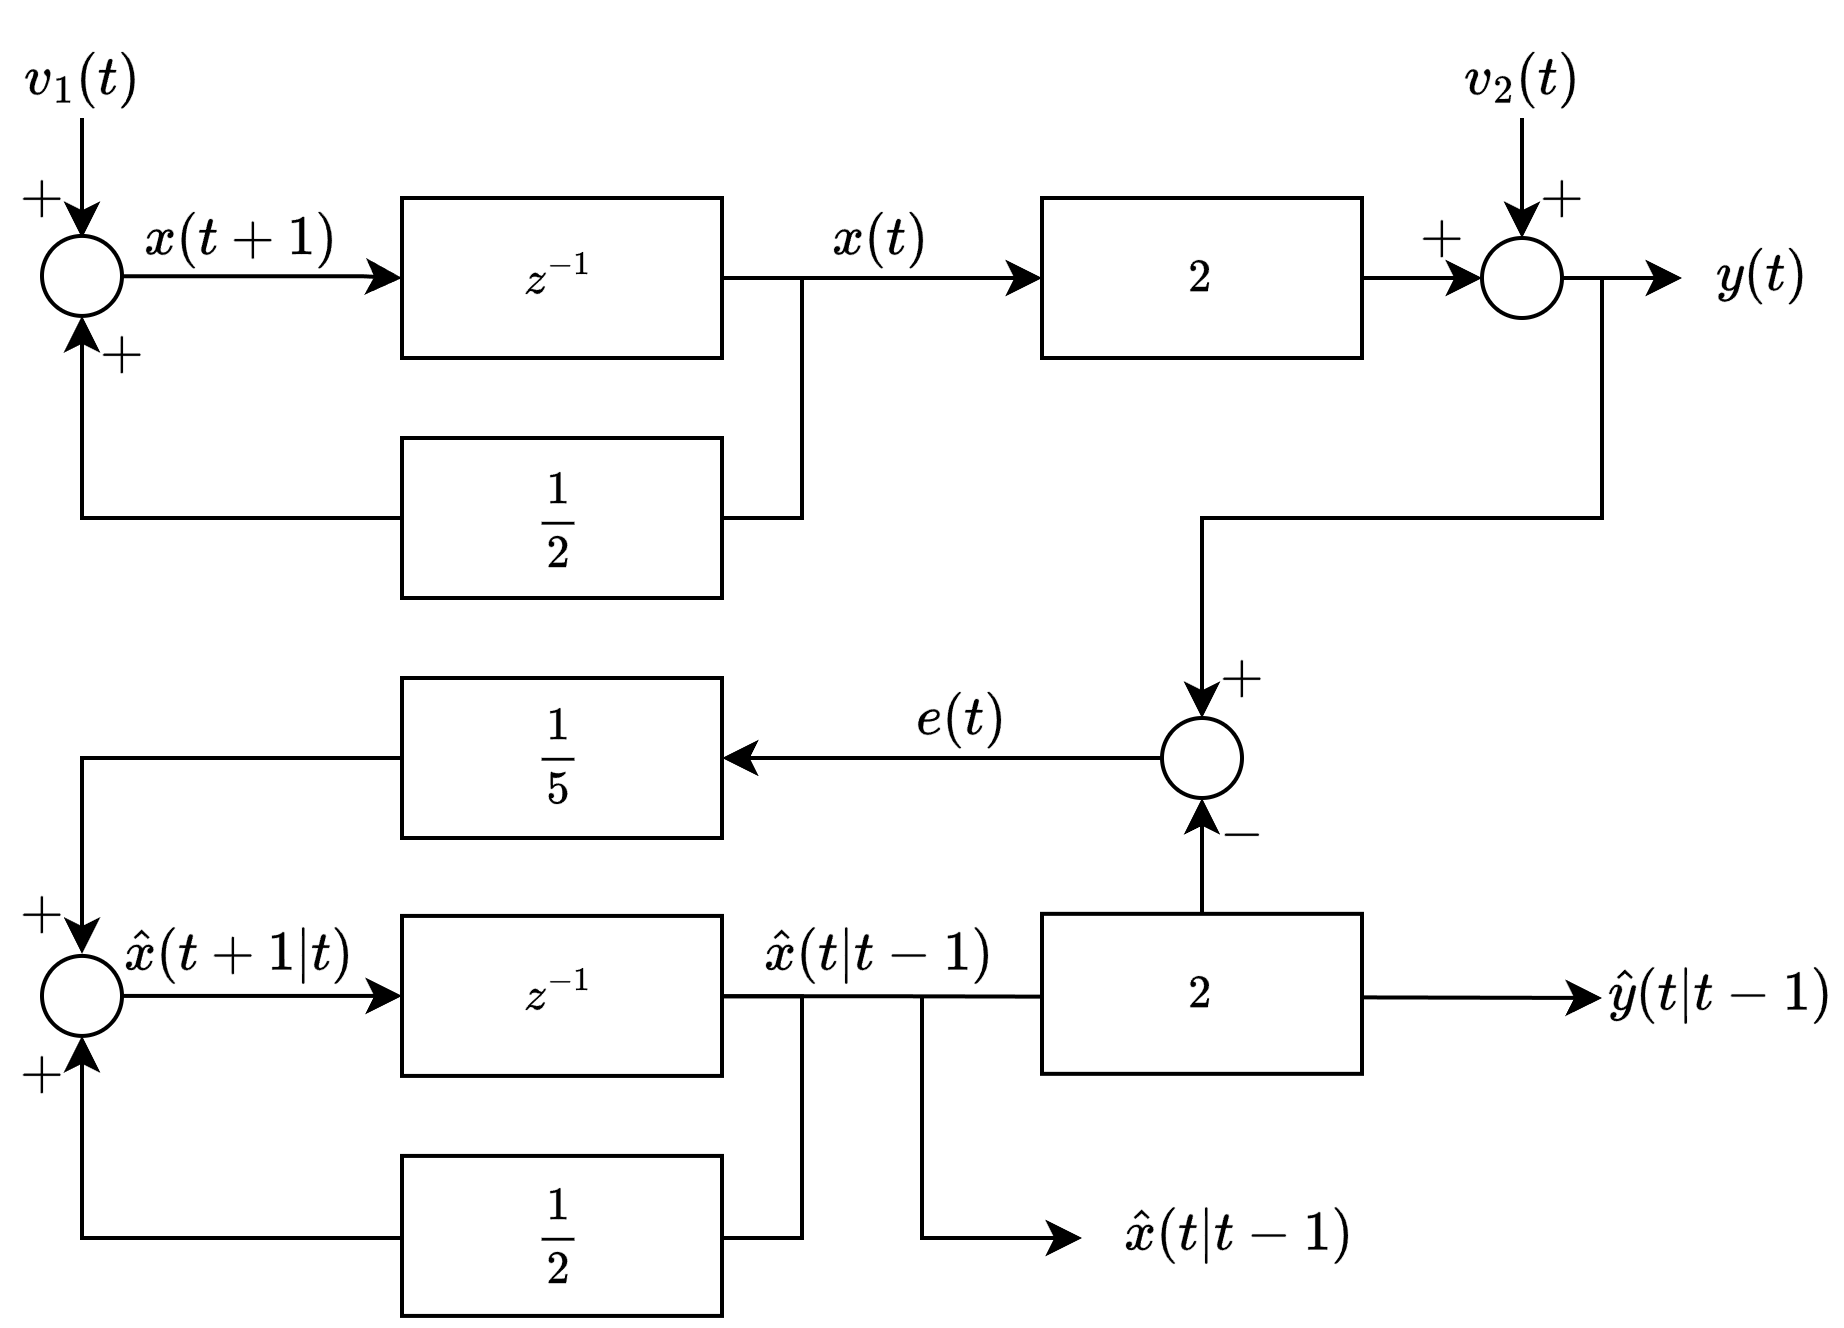
\includegraphics[width=0.6\linewidth]{images/block3.png}
            \end{figure}
            From the block diagram, we can derive the transfer function for the state estimate as:
            \[\hat{x}(t|t-1)=\dfrac{\frac{1}{5}\frac{z^{-1}}{1-\frac{1}{2}z^{-1}}}{1+\frac{1}{5}\frac{z^{-1}}{1-\frac{1}{2}z^{-1}}\cdot 2}=\dfrac{\frac{1}{5}}{1-\frac{1}{10}z^{-1}}y(t-1)\]
            The prediction of the output is then given by:
            \[\hat{y}(t|t-1)=H\hat{x}(t|t-1)=\dfrac{\frac{2}{5}}{1-\frac{1}{10}z^{-1}}y(t-1)\]
    \end{enumerate}
    The filter is determined as follows:
    \[\hat{x}(t|t)=F^{-1}\hat{x}(t+1|t)=\dfrac{\frac{2}{5}}{1-\frac{1}{10}z^{-1}}y(t)\]
\end{example}